\documentclass[11pt,aspectratio=169,dvipsnames]{beamer}
\graphicspath{{figs/}}
\usetheme{default}
\usepackage{DasBeamerPaket}
\usepackage{animate}
\usepackage{lastpage}
\usepackage{appendixnumberbeamer}
\usepackage{braket}
\usepackage{booktabs}
\usepackage{tabularx}
\usepackage{tikz}
\usepackage{eso-pic}
\setbeamercolor{section in toc}{fg=NavyBlue}
\setbeamercolor{frametitle}{fg=NavyBlue}
\captionsetup[figure]{labelfont=bf}
\captionsetup[table]{labelfont=bf}
\newcommand{\theauthor}{Jakob Krause}
\newcommand{\theshortauthor}{\textsc{J. Krause} for CBELSA/TAPS}
\newcommand{\authormail}{krause@hiskp.uni-bonn.de}
\newcommand{\authorgit}{krausejm}
\newcommand{\thetitle}{Determination of the beam asymmetry $\Sigma$  in $\eta$- and $\eta'$-photoproduction off the proton using Bayesian statistics}
\newcommand{\theshorttitle}{$\Sigma$ in $\eta$- and $\eta'$ photoproduction}
\newcommand{\thecolor}{black!70!blue}
\newcommand{\thecolorr}{black!60!blue}
\newcommand{\thecolorrr}{black!50!blue}
\newcommand{\thesubtitle}{Master thesis for the CBELSA/TAPS collaboration}
\newcommand{\thedate}{September 8/9 2022}
\makeatletter
\patchcmd{\beamer@calculateheadfoot}{\advance\footheight by 4pt}{\advance\footheight by 20pt}{}{}
\makeatother

\begin{document}
	\definecolor{myWhite}{rgb}{1,1,1}
	
	
	\setbeamercolor{coloredboxstuff}{fg=myWhite,bg=\thecolor}
	\setbeamercolor{coloredboxstuff1}{fg=myWhite,bg=\thecolorr}
	\setbeamercolor{coloredboxstuff2}{fg=myWhite,bg=\thecolorrr}	
	
	
	\makeatother
	\setbeamertemplate{footline}
	{
		\leavevmode%
		\hbox{%
			\begin{beamercolorbox}[wd=.34\paperwidth,ht=2.25ex,dp=1ex,center]{coloredboxstuff}%
				{\theshortauthor}
			\end{beamercolorbox}%
			\begin{beamercolorbox}[wd=.34\paperwidth,ht=2.25ex,dp=1ex,center]{coloredboxstuff1}%
				{\theshorttitle}
			\end{beamercolorbox}%
			\begin{beamercolorbox}[wd=.34\paperwidth,ht=2.25ex,dp=1ex,center]{coloredboxstuff}%
				\insertframenumber{} / \inserttotalframenumber\hspace*{1ex}
		\end{beamercolorbox}}%
	}
	\makeatletter
	
	
	\setbeamercovered{transparent}
	\setbeamertemplate{navigation symbols}{}
	\setbeamertemplate{frametitle}[default][left,leftskip=0.5cm]
	\setbeamertemplate{itemize item}{\color{black}$\blacktriangleright$}
	\setbeamertemplate{section in toc}[sections numbered]
	\setbeamercolor{section in toc}{fg=\thecolor}
	\setbeamercolor{frametitle}{fg=\thecolor}
	\captionsetup{font=scriptsize,labelfont=scriptsize}
	\setbeamercovered{invisible}
	\AtBeginSection[]{
	\ifnum \thesection=3
	\else
	\begin{frame}
		\tableofcontents[currentsection] 
	\end{frame} 
	\fi
}
\AtBeginSubsection[]{

	\begin{frame}
		\tableofcontents[currentsection,currentsubsection] 
	\end{frame} 
}

	
	
	
	\begin{frame}[plain,noframenumbering]
		\begin{tikzpicture}[remember picture,overlay]
			\node[anchor= north east] at (current page.north east) {
\includegraphics[width=2.5cm]{logo}};
		\end{tikzpicture}
		\centering
		{\Large \color{\thecolor}{\thetitle}}\\
		\vspace{0.5cm}
		{\thesubtitle}
		\vfill
		\begin{minipage}{\linewidth}
			\centering
			\begin{minipage}{\linewidth}
				\centering
				\textsc{\theauthor}\\
				\scriptsize \href{mailto:\authormail}{\faEnvelope  \hspace*{0.1cm}\authormail} {\color{black}$|$} \href{https://github.com/\authorgit}{\faGithub  \hspace*{0.1cm}\authorgit}\\
			\end{minipage}
			\vspace{.5cm}
			
			{\scriptsize
				Supervisor: \textsc{Jun. Prof. Dr. Annika Thiel}\\
				\tiny \href{mailto:thiel@hiskp.uni-bonn.de}{\faEnvelope  \hspace*{0.1cm}thiel@hiskp.uni-bonn.de}\par}
		\end{minipage}
		\vspace{0.2cm}
		
		\thedate
	\end{frame}
	
	
	\begin{frame}{Setting the scene}
		\setcounter{page}{1}
		\begin{tcolorbox}[colback=blue!5,colframe=\thecolor,title=The Standard Model of Particle Physics]
			\begin{itemize}
				\item matter consists of 12 (anti-)\emph{fermions}
				\item quarks interact via \emph{strong interaction} 
				\item form bound states: mesons ($q\bar{q}$) and baryons ($qqq$)
			\end{itemize} 
		\end{tcolorbox}
		baryon spectroscopy (photoproduction) gives insight in strong interaction
		\begin{center}
			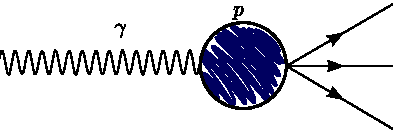
\includegraphics[width=.6\linewidth]{feynman}
		\end{center}
		
		
		
		
	\end{frame}
	\begin{frame}{Setting the scene}
		Observe resonances $N^*/\Delta^*$ in the cross sections $\sigma(\gamma p\to p M)$
		\vspace{-0.5cm}
		\begin{figure}
			\centering
			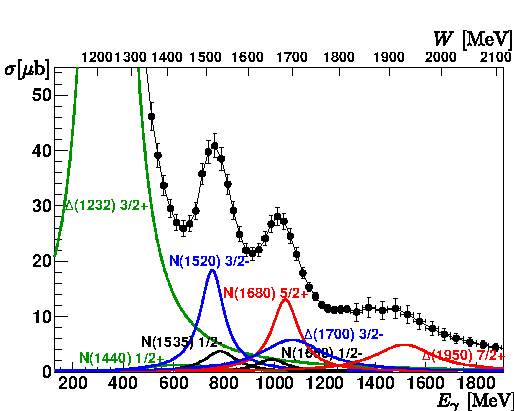
\includegraphics[width=.5\linewidth]{partialwaves}
			\caption*{Total cross section $\sigma(\gamma p\to p \pi^0)$ \citef{wuafzth}}
		\end{figure}
		$\to$goal: (help to) identify contributing resonances as strong bound states!\\
	\end{frame}

	\begin{frame}
		\setcounter{tocdepth}{2}
		\tableofcontents
	\end{frame}
\section{Theoretical basics}
	\begin{frame}{Theoretical basics I}
		\begin{itemize}
			\item resonances are broad, overlapping, require complicated partial-wave-analysis (PWA)
			\item constraints for the analysis can be derived from polarization observables
			\item ultimate goal: "complete experiment"; unambiguous, model-independent PWA solution $\to$ several single and double polarization observables needed
		\end{itemize}
		\begin{tcolorbox}[colback=blue!5,colframe=\thecolor,title = Beam-target polarization observables]
			\centering
			\begin{tabularx}{.7\linewidth}{|l|l|X|X|X|}
				\hline
				\multicolumn{2}{|c}{}&\multicolumn{3}{c|}{\textbf{target polarization}}\\
				\textbf{photon} & &$x$&$y$&$z$\\
				\hline
				unpolarized & $\sigma_0$&-&$T$&-\\
				linearly polarized &\color{red}{$-\Sigma$}&$H$&$-P$&$-G$\\
				circularly polarized &-&$F$&-&$-E$\\
				\hline
			\end{tabularx}
			\begin{flushright}
				\cites{san}
			\end{flushright}
		\end{tcolorbox}	
	\end{frame}
	
	
	
\begin{frame}{Theoretical basics I}
		
		
		
		\begin{tcolorbox}[colback=blue!5,colframe=\thecolor,title=Beam asymmetry $\boldsymbol{\Sigma}$]
			$$\frac{\text{d}\sigma}{\text{d}\Omega}(E_\gamma,\cos\theta,\varphi)=\frac{\text{d}\sigma}{\text{d}\Omega}_0(E_\gamma,\cos\theta)\cdot\left[1-p_\gamma^{\text{lin}}\boldsymbol{\Sigma}\cos(2\varphi)\right]$$
			polarization angle $\varphi$, polarization degree $p_\gamma^{\text{lin}}$
			\begin{flushright}
				{\scriptsize[\cite{san}]}
			\end{flushright}
		\end{tcolorbox}
		
		\begin{figure}
			\centering
			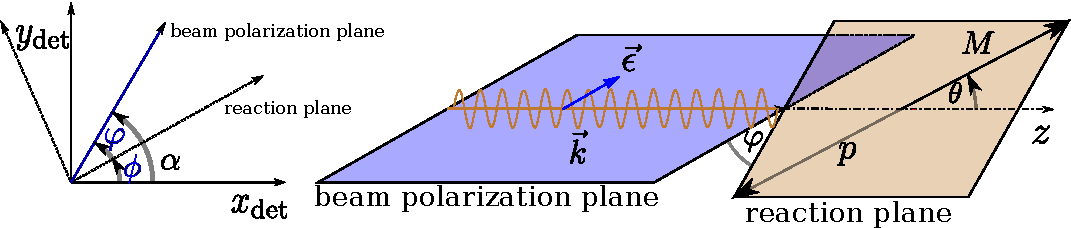
\includegraphics[width=.8\linewidth]{angles.pdf}
			\caption*{Definition of the polarization angle}
		\end{figure}
	\end{frame}
	\begin{frame}{Theoretical basics II}
	\begin{itemize}
		\item Polarization observables are input for further analysis
		\item Idea: increase amount of information gained from results using \textsc{Bayesian} inference 
	\end{itemize}
	\begin{tcolorbox}[colback=blue!5,colframe=\thecolor,title=\textsc{Bayes'} theorem]
		\begin{align*}
			p(\theta|y)&\propto p(y|\theta)\cdot p(\theta)\\
			\text{\emph{posterior}}&\propto\text{\emph{likelihood}}\cdot\text{\emph{prior}}
		\end{align*}
		parameters $\theta$ and data $y$.
		
		
		\begin{flushright}
			{\scriptsize[\cite{bayes}]}
		\end{flushright}
	\end{tcolorbox}
	\end{frame}

	\begin{frame}{Theoretical basics II}
		\addtocounter{framenumber}{-1}
	\begin{itemize}
		\item Polarization observables are input for further analysis
		\item Idea: increase amount of information gained from results using \textsc{Bayesian} inference 
	\end{itemize}
	\begin{tcolorbox}[colback=blue!5,colframe=\thecolor,title=\textsc{Bayes'} theorem]
		\begin{align*}
			p(\theta|y)&\propto p(y|\theta)\cdot p(\theta)\\
			\text{\emph{posterior}}&\propto\text{\emph{likelihood}}\cdot\text{\emph{prior}}
		\end{align*}
	parameters $\theta$ and data $y$.
	
	
	\begin{flushright}
		{\scriptsize[\cite{bayes}]}
	\end{flushright}
\end{tcolorbox}
\AddToShipoutPictureFG*{%
	\begin{tikzpicture}[remember picture,overlay]
		\node at (current page.center) {
\includegraphics[width=.4\linewidth]{confused_man}};
	\end{tikzpicture}
}

	\end{frame}

\begin{frame}{Theoretical basics II}
			\addtocounter{framenumber}{-1}
	$$p(\theta|y)\propto p(y|\theta)\cdot p(\theta)$$
		\begin{itemize}
			\item prior $p(\theta)$ and likelihood $p(y|\theta)$ can easily be specified \\
			$\to$ gain \emph{distributions} $p(\theta|y)$ instead of point estimates with error bars
		\end{itemize}
		\begin{tcolorbox}[colback=blue!5,colframe=\thecolor,title=\textsc{Bayesian} parameter inference]
			For each parameter $\theta_n\in\theta$ we gain \emph{marginal posteriors}
			\begin{equation*}
				\label{eq:marpost}
				p(\theta_n|y)=\int\text{d}\theta_1\dots\int\text{d}\theta_{n-1}\int\text{d}\theta_{n-1}\dots\int\text{d}\theta_Np(\theta_1\dots\theta_N|y).
			\end{equation*}
		usually approximated using \textsc{Markov}-Chain Monte Carlo (MCMC) draws $\theta^{(s)}$
			\begin{flushright}
				{\scriptsize[\cite{sivia}]}
			\end{flushright}
		\end{tcolorbox}
	\end{frame}
	\begin{frame}{Theoretical basics II}
		$$p(\theta|y)\propto p(y|\theta)\cdot p(\theta)$$
		\begin{itemize}
			\item prior $p(\theta)$ and likelihood $p(y|\theta)$ can easily specified \\
			$\to$ gain \emph{distributions} $p(\theta|y)$ instead of point estimates with error bars
		\end{itemize}
		\begin{tcolorbox}[colback=blue!5,colframe=\thecolor,title=\textsc{Bayesian} parameter inference]
			For each parameter $\theta_n\in\theta$ we gain \emph{marginal posteriors}
			\begin{equation*}
				\label{eq:marpost}
				p(\theta_n|y)=\int\text{d}\theta_1\dots\int\text{d}\theta_{n-1}\int\text{d}\theta_{n-1}\dots\int\text{d}\theta_Np(\theta_1\dots\theta_N|y).
			\end{equation*}
			usually approximated using \textsc{Markov}-Chain Monte Carlo (MCMC) draws $\theta^{(s)}$
			\begin{flushright}
				{\scriptsize[\cite{sivia}]}
			\end{flushright}
		\end{tcolorbox}
	\AddToShipoutPictureFG*{%
		\begin{tikzpicture}[remember picture,overlay]
			\node at (current page.center) {
\includegraphics[width=.4\linewidth]{idea_man}};
		\end{tikzpicture}
	}
	\end{frame}
	\section{Experimental Setup}
	\begin{frame}{CBELSA/TAPS experiment}
		\begin{minipage}{.3\linewidth}
			{\small
				\begin{itemize}
					\item generate photon beam from accelerated electrons via bremsstrahlung, with $E_\gamma\leq\SI{3.2}{\giga\eV}$ 
					\item photon beam impinges on liquid hydrogen target: $\gamma p \to p M\to p X$
					\item measure decay products $X$ of different final states: $M=\pi^0/\eta/\eta'/\dots$
					\item data set: July-October 2013, 1065 h beam time
				\end{itemize}
			}
		\end{minipage}
		\begin{minipage}{.69\linewidth}
			\begin{figure}
				\centering
				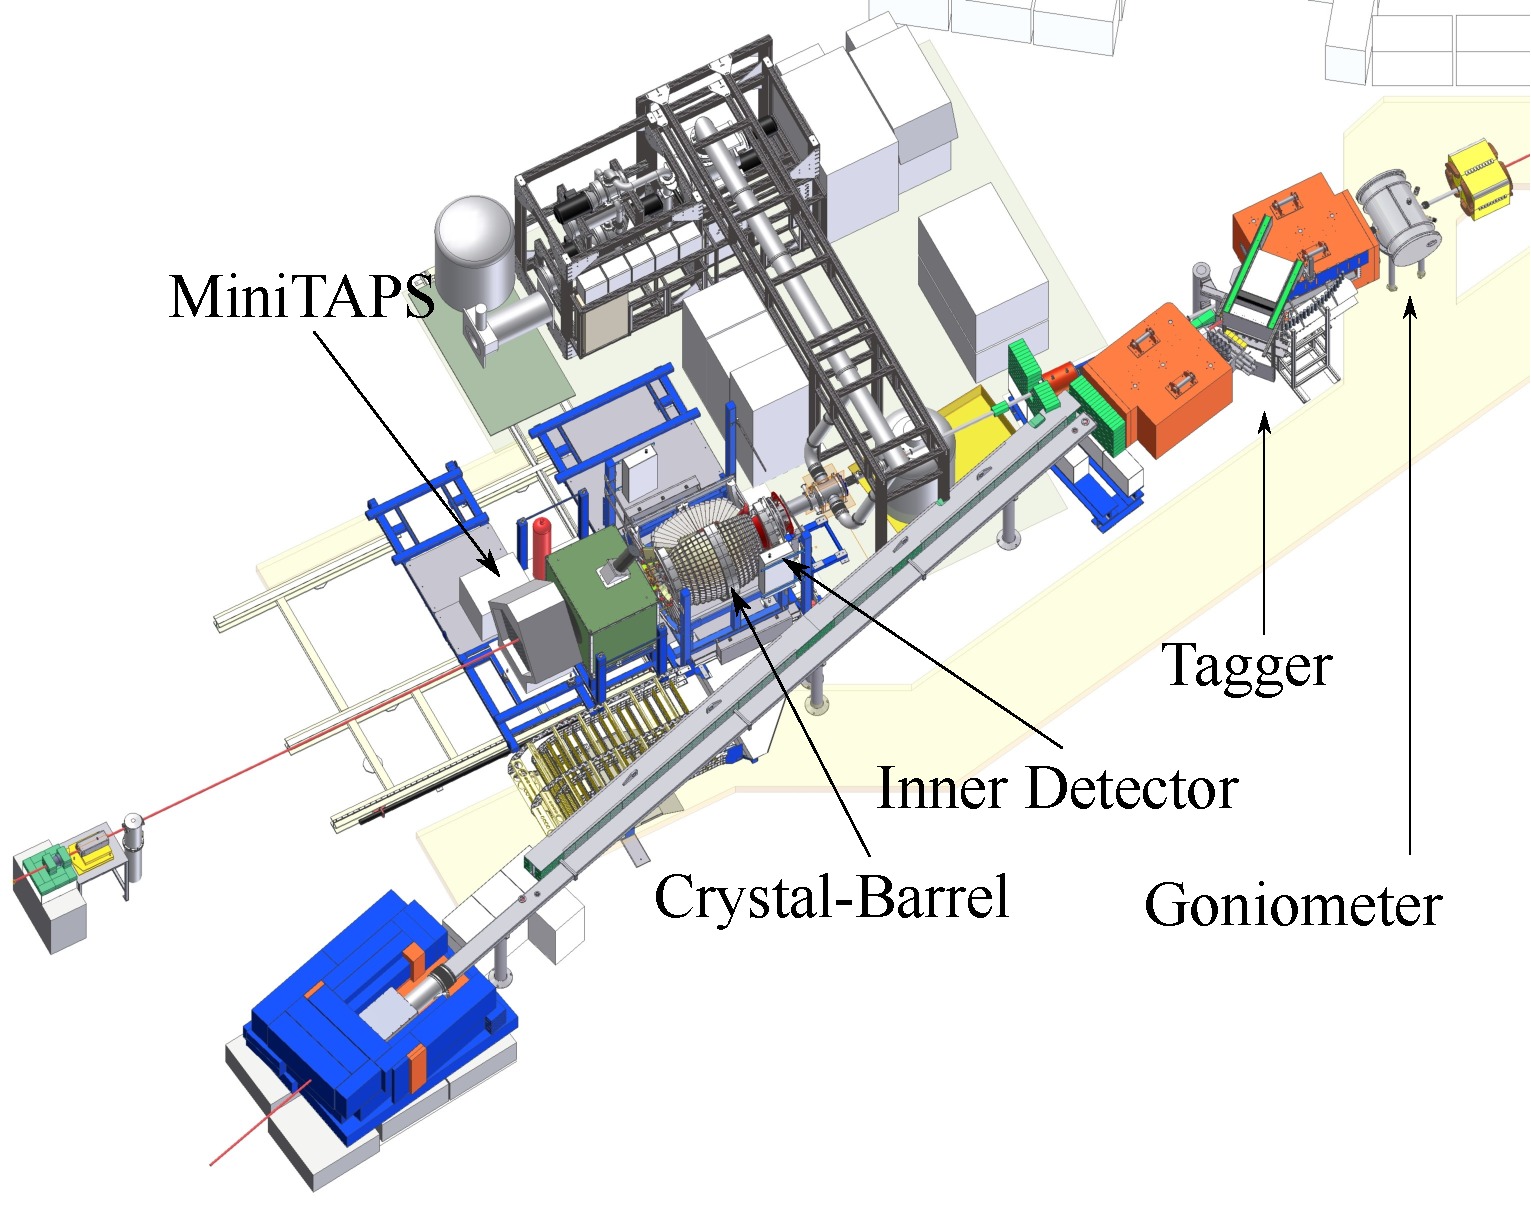
\includegraphics[width=.9\linewidth]{CB-Area}
				\caption*{Overview of the experimental area, adapted from \citef{cb}}
			\end{figure}
		\end{minipage}
		
	\end{frame}

	
	
	\section{Results}
	\subsection{Determination of $\Sigma_\eta$ using \textsc{Bayesian} statistics}
		\begin{frame}{Confirming pre-published results of $\Sigma_\eta$}
		\begin{itemize}
			\item Polarization observables are needed for different final states ($\pi^0,{\color{red}\eta},\eta',\dots$)
			\item high precision measurement of beam asymmetry for $\eta$ production recently published {\cites{eta}}
			\item goal: confirm results using \textsc{Bayesian} fitting methods
		\end{itemize}
		
	\end{frame}
	\begin{frame}{Confirming pre-published results for $\Sigma_\eta$}
		
		\begin{minipage}{\linewidth}
			\begin{tcolorbox}[colback=blue!5,colframe=\thecolor,title={Event selection ($\eta$)}]
				analysis performed in 11x12 bins of $(E_\gamma,\cos\theta)$ for $\gamma p\to p\eta\to p\gamma\gamma$ by {\cites{eta}}
			\end{tcolorbox}
		\end{minipage}
		\begin{minipage}{\linewidth}
			\begin{tcolorbox}[colback=blue!5,colframe=\thecolor,title={Methods}]
				\begin{center}
					Remember: $\frac{\text{d}\sigma}{\text{d}\Omega}(E_\gamma,\cos\theta,\varphi)=\frac{\text{d}\sigma}{\text{d}\Omega}_0(E_\gamma,\cos\theta)\cdot\left[1-p_\gamma^{\text{lin}}\boldsymbol{\Sigma}\cos(2\varphi)\right]$
				\end{center}
				

					\begin{tcolorbox}[colback=blue!5,colframe=\thecolor,title={Binned fit to event yield asymmetries}]
					fit to event yield asymmetries $A(E_\gamma,\theta,\phi)$\\ $$=\frac{N^\bot(E_\gamma,\theta,\phi)-N^\parallel(E_\gamma,\theta,\phi)}{p_\gamma^\parallel N^\bot(E_\gamma,\theta,\phi) + p_\gamma^\bot N^\parallel(E_\gamma,\theta,\phi)}=\Sigma(E_\gamma,\theta)\cos\left(2\left(\alpha^\parallel-\phi\right)\right)$$
							
					\end{tcolorbox}		
					
			\end{tcolorbox}
		\end{minipage}
	\end{frame}
	\begin{frame}[noframenumbering]{Confirming pre-published results for $\Sigma_\eta$}
	
	\begin{minipage}{\linewidth}
			\begin{tcolorbox}[colback=blue!5,colframe=\thecolor,title={Event selection ($\eta$)}]
		analysis performed in 11x12 bins of $(E_\gamma,\cos\theta)$ for $\gamma p\to p\eta\to p\gamma\gamma$ by {\cites{eta}}
	\end{tcolorbox}
	\end{minipage}
	\begin{minipage}{\linewidth}
		\begin{tcolorbox}[colback=blue!5,colframe=\thecolor,title={Methods}]
			\begin{center}
				Remember: $\frac{\text{d}\sigma}{\text{d}\Omega}(E_\gamma,\cos\theta,\varphi)=\frac{\text{d}\sigma}{\text{d}\Omega}_0(E_\gamma,\cos\theta)\cdot\left[1-p_\gamma^{\text{lin}}\boldsymbol{\Sigma}\cos(2\varphi)\right]$
			\end{center}
			
			
			\begin{tcolorbox}[colback=blue!5,colframe=\thecolor,title={Unbinned maximum likelihood fit}]
				Consider likelihood of each individual event

					$$\tilde{p}(\phi,\Sigma)=\frac{\left(1+p_\gamma\Sigma\cos\left(2\left(\alpha^\parallel-\phi\right)\right)\right)\cdot\epsilon\left(\phi\right)}{C}$$
				
			\end{tcolorbox}		
			
		\end{tcolorbox}
	\end{minipage}
\end{frame}
	\begin{frame}{Confirming pre-published results for $\Sigma_\eta$}
		Applying \textsc{Bayesian} approach to event yield asymmetries:
		\begin{itemize}
			\item assume \textsc{Gaussian} errors, i.e.
			$$A(\phi)=\Sigma\cos\left(2\left(\alpha^\parallel-\phi\right)\right)+\epsilon$$ where $\epsilon\sim\mathcal{N}(0,\sigma)$
			\item likelihood $p(A|\Sigma)$ of each datapoint given by $$y\sim\mathcal{N}\left(\Sigma\cos\left(2\left(\alpha^\parallel-\phi\right)\right),\sigma\right)$$
			\item prior: $$p(\Sigma)\sim\mathcal{N}(0,1)_{[-1,1]}$$
		\end{itemize}
	Sample from posterior $p(\Sigma|A)\propto p(A|\Sigma)\cdot p(\Sigma)$ !
	\end{frame}
		\begin{frame}{Confirming pre-published results for $\Sigma_\eta$}
		Applying \textsc{Bayesian} approach to unbinned fit:
		\begin{itemize}
			\item event based likelihood given by product of all single-event likelihoods 
			\item assign priors for all fit parameters (18 in total)
			\item truncate beam asymmetry to allowed region $[-1,1]$
			\item perform toy Monte Carlo experiments
		\end{itemize}
		Sample from posterior !
	\end{frame}
	
	\begin{frame}{Confirming pre-published results for $\Sigma_\eta$}
		\begin{itemize}
			\item All \textsc{Bayesian} fits performed using the \emph{Python} frontend of \emph{Stan}
			\item MCMC-sampling: adaptive \textsc{Hamiltonian} Monte-Carlo (HMC), i.e. No-U-Turn-Sampling (NUTS)
			\begin{itemize}
				\item generate samples $\theta^{(1)},\theta^{(2)},\dots,\theta^{(S)}$ where each $\theta^{(t)}$ depends only on $\theta^{(t-1)}$
				\item simulate draws from the posterior by updating at point $t$ such that the posterior increases (importance sampling)
			\end{itemize}
		\item diagnosing convergence of MCMC:
		\begin{itemize}
			\item potential scale reduction statistic $1.00\lesssim\widehat{R}\lesssim1.01$
			\item Monte Carlo standard error (MCSE) \enquote{small}
		\end{itemize}
			\item Goodness of fit: posterior predictive checks (PPC)
		\end{itemize}

	\begin{flushright}
		
\includegraphics[width=.1\linewidth]{figs/logo-tm.png}\\
		\cites{stan,nuts}
	\end{flushright}
	\end{frame}
\begin{frame}{Confirming pre-published results for $\Sigma_\eta$}
	PPC for \emph{binned} \textsc{Bayesian} fit:
	\centering
	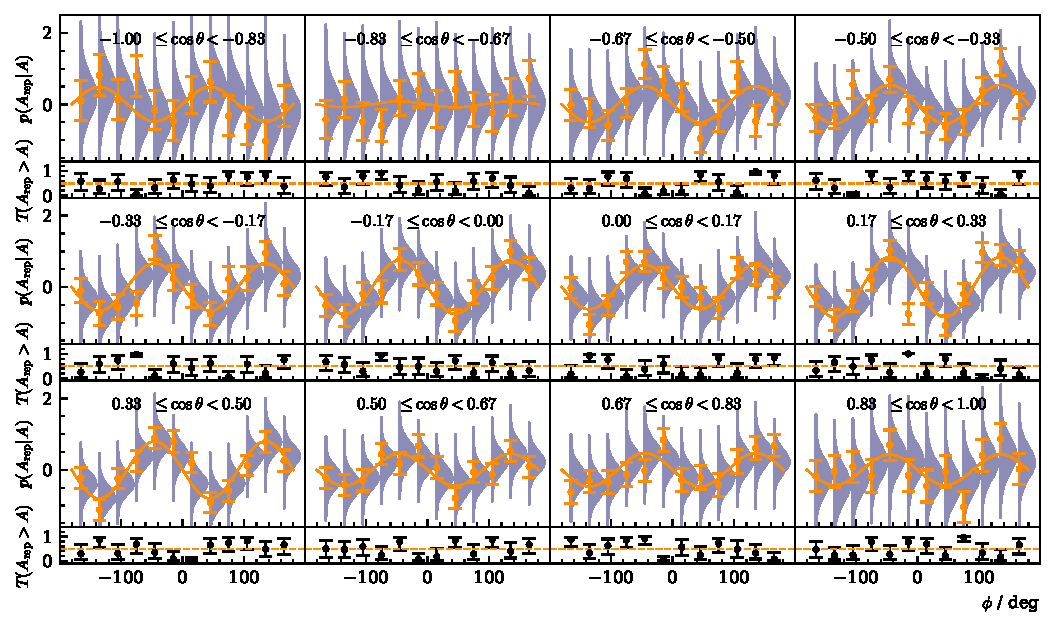
\includegraphics[width=.9\linewidth]{../../bayes/realdeal/plots/ppd_checks.pdf}
\end{frame}
\begin{frame}{Confirming pre-published results for $\Sigma_\eta$}
	PPC for \emph{unbinned} \textsc{Bayesian} fit:
	\centering
	
\includegraphics[width=.9\linewidth]{../../bayes/event_based_fit/plots/eff_PPC.png}
\end{frame}
\begin{frame}{Confirming pre-published results for $\Sigma_\eta$}
	\begin{figure}
		\centering
		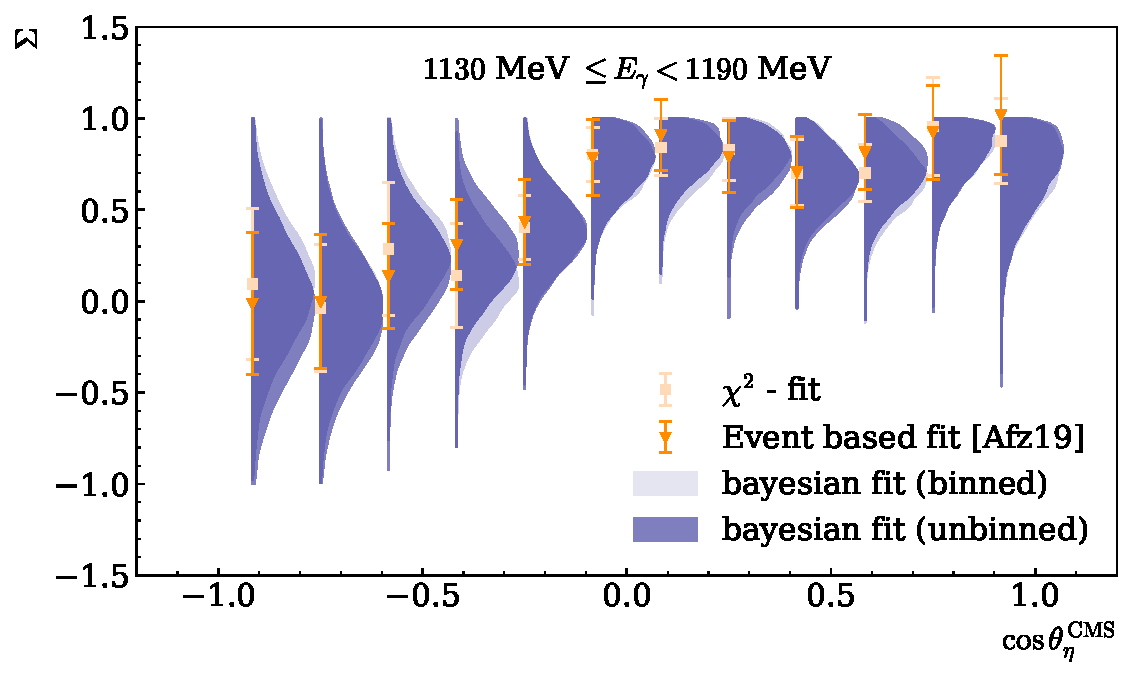
\includegraphics[width=.8\linewidth]{../../bayes/event_based_fit/plots/sigma_eta_bin.pdf}
	\end{figure}
	Distinct advantage: sample only in physically allowed parameter space
\end{frame}
	\begin{frame}{Confirming pre-published results for $\Sigma_\eta$}
		\begin{figure}
			\centering
			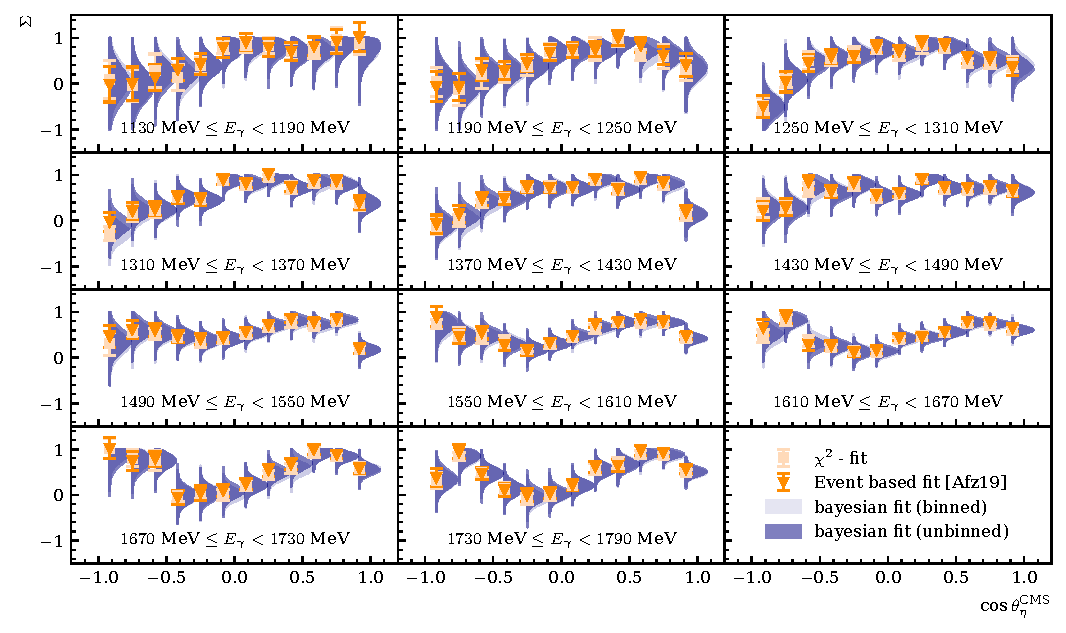
\includegraphics[width=.95\linewidth]{../../bayes/event_based_fit/plots/sigma_eta.pdf}
		\end{figure}
	\end{frame}
	
	
	
	
	\subsection{Determination of $\Sigma_{\eta'}$}
	
	\begin{frame}{Determining the beam asymmetry in $\eta'$ photoproduction}
		First, perform event selection regarding $\eta'$ photoproduction
		\begin{table}
\centering
\begin{tabular}{cc}
	\toprule
	\multicolumn{2}{c}{$\eta'$}\\
	\hline
	Decay mode&Branching ratio\\
	\hline
	$\pi^+\pi^-\eta$&42.6\%\\
	$\rho^0\gamma(\to\pi^+\pi^-\gamma)$ &28.9\% (28.9\%)\\
	$\pi^0\pi^0\eta(\to6\gamma$) & 22.8\% (8.8\%)\\
	$\omega\gamma(\to \pi^+\pi^-\pi^0\gamma/\pi^0\gamma\gamma)$&2.52\% (2.2\%/0.21\%)\\
	$\gamma\gamma$&2.3\%\\
	\bottomrule
\end{tabular}
		\end{table}
		\begin{flushright}
			\cites{pdg}
		\end{flushright}
	\end{frame}
	\begin{frame}[noframenumbering]{Determining the beam asymmetry in $\eta'$ photoproduction}
	First, perform event selection regarding $\eta'$ photoproduction
	\begin{table}
		\centering
		\begin{tabular}{cc}
			\toprule
			\multicolumn{2}{c}{$\eta'$}\\
			\hline
			Decay mode&Branching ratio\\
			\hline
			$\pi^+\pi^-\eta$&42.6\%\\
			$\rho^0\gamma(\to\pi^+\pi^-\gamma)$ &28.9\% (28.9\%)\\
			$\pi^0\pi^0\eta(\to6\gamma$) & 22.8\% (8.8\%)\\
			$\omega\gamma(\to \pi^+\pi^-\pi^0\gamma/\pi^0\gamma\gamma)$&2.52\% (2.2\%/0.21\%)\\
			\arrayrulecolor{red}
			\hline
			\multicolumn{1}{!{\color{red}\vline}c}{$\gamma\gamma$}&\multicolumn{1}{c!{\color{red}\vline}}{2.3\%}\\
			\hline
			\arrayrulecolor{black}
			\bottomrule
		\end{tabular}
	\begin{flushright}
		\cites{pdg}
	\end{flushright}
	\end{table}
	
\end{frame}	

\begin{frame}{Determining the beam asymmetry in $\eta'$ photoproduction}
	\begin{tcolorbox}[colback=blue!5,colframe=\thecolor,title={Event selection ($\eta'$)}]
		analysis performed in 3x6 bins of $(E_\gamma,\cos\theta)$ for $\gamma p\to p\eta'\to p\gamma\gamma$,\\ $E_\gamma\in[1500,1800]$ MeV
		\vspace{-0.5cm}
		\begin{align*}
			&p_\gamma + p_p &&= p_{\eta'}+p_\text{recoil}& &=\underbrace{p_{\gamma_1}+p_{\gamma_2}}_{=p_{\eta'}}+p_\text{recoil}\\
			&p_\gamma + p_p &&= p_{\eta'}+p_X &&=\underbrace{p_{\gamma_1}+p_{\gamma_2}}_{=p_{\eta'}} + p_X
		\end{align*}
		\vspace{-0.7cm}
		\begin{itemize}
			\item one charged, two uncharged detector hits in coincidence with beam $\gamma$
			\item Coplanarity $\Delta\phi=\phi_{\eta'}-\phi_\text{recoil}\overset{!}{=}\SI{180}{\degree}$
			\item Polar angle $\theta_X\overset{!}{=}\theta_\text{recoil}$
			\item Missing mass $m_X\overset{!}{=}m_p$
			\item Invariant mass $m_{\gamma\gamma}\overset{!}{=}m_{\eta'}$
		\end{itemize}
	\end{tcolorbox}
\end{frame}

\begin{frame}{Determining the beam asymmetry in $\eta'$ photoproduction}
	\vspace{-0.95cm}
	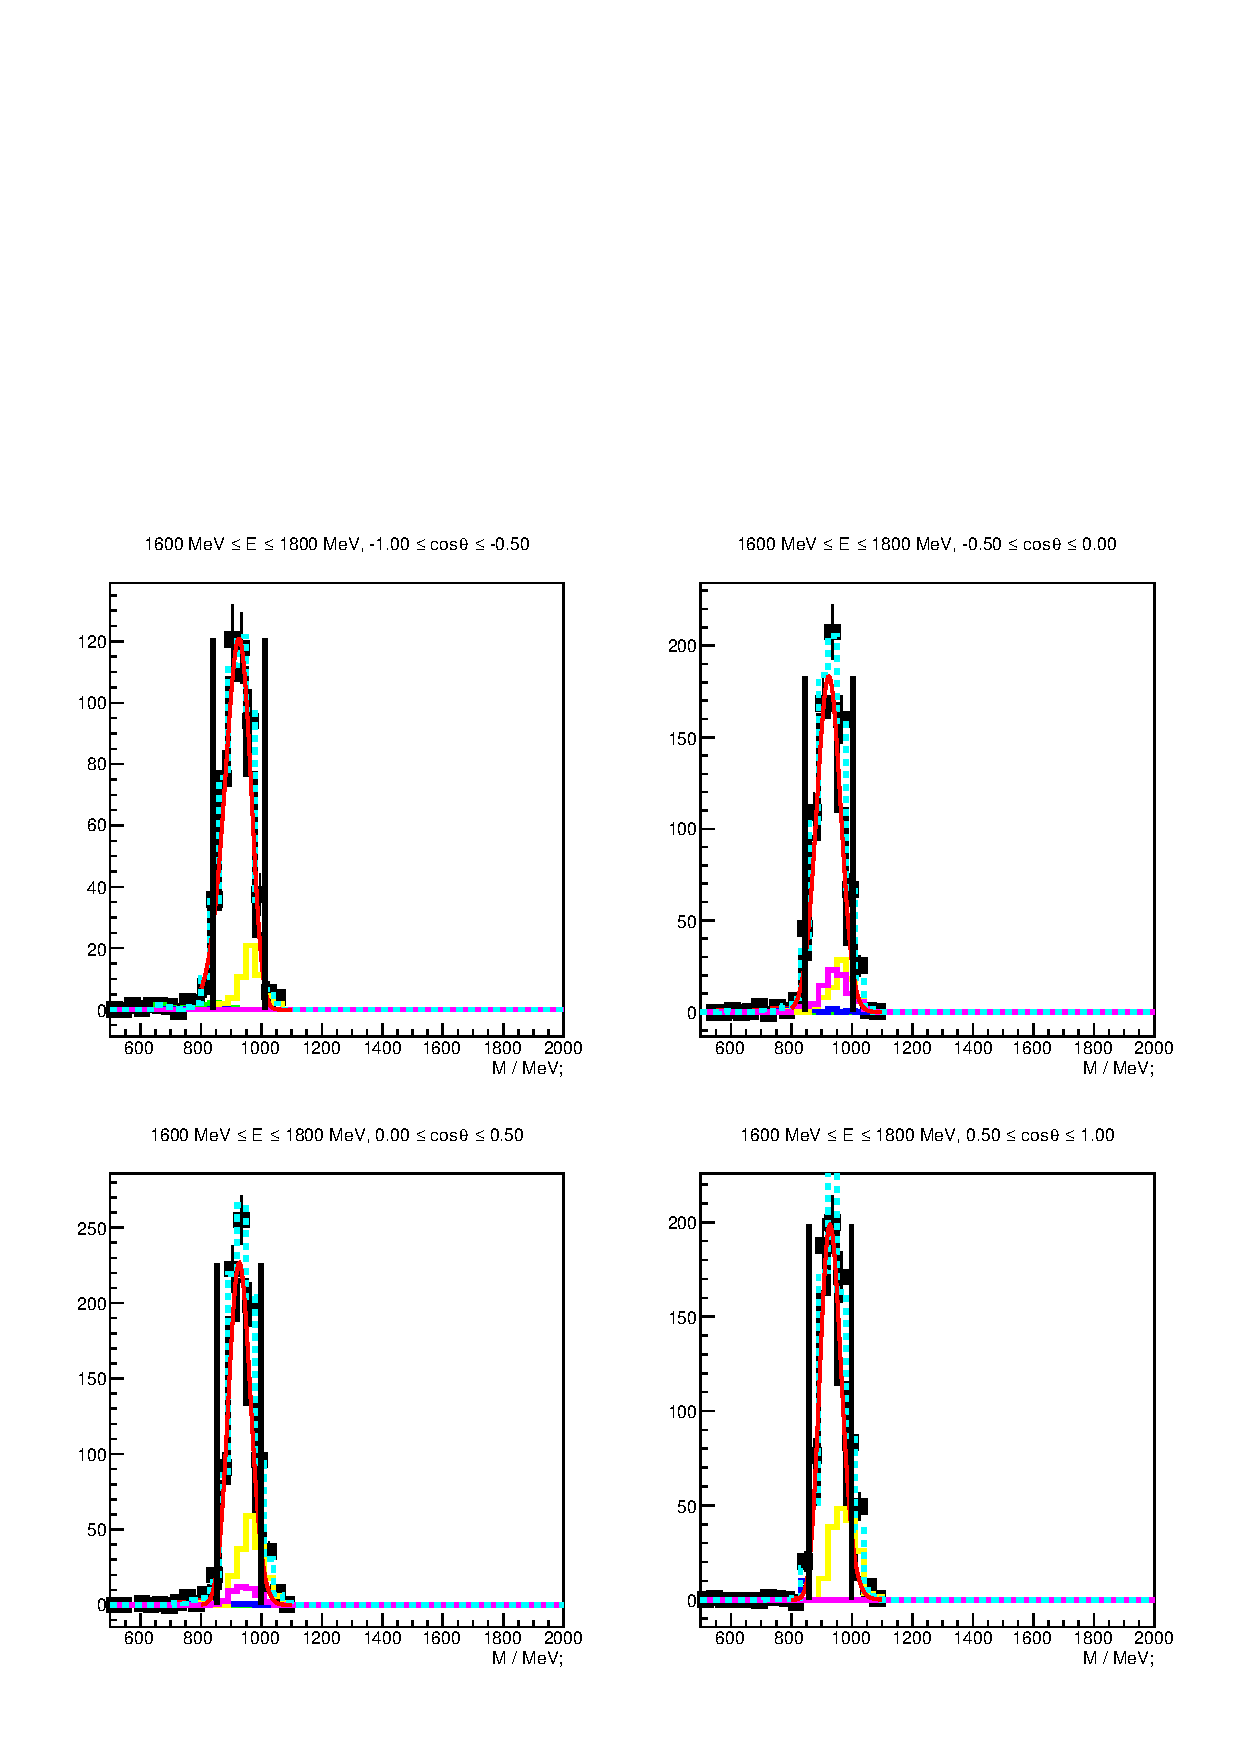
\includegraphics[width=.95\linewidth]{../../figs/hydrogen/bin_cuts/mismcut_ebin1.pdf}
	data points: $m_X$, turquoise: total MC, black: $\eta'$ MC, yellow: $2\pi^0$ MC, magenta: $\pi^0\eta$ MC
\end{frame}
\begin{frame}{Determining the beam asymmetry in $\eta'$ photoproduction}
	\vspace{-0.95cm}
	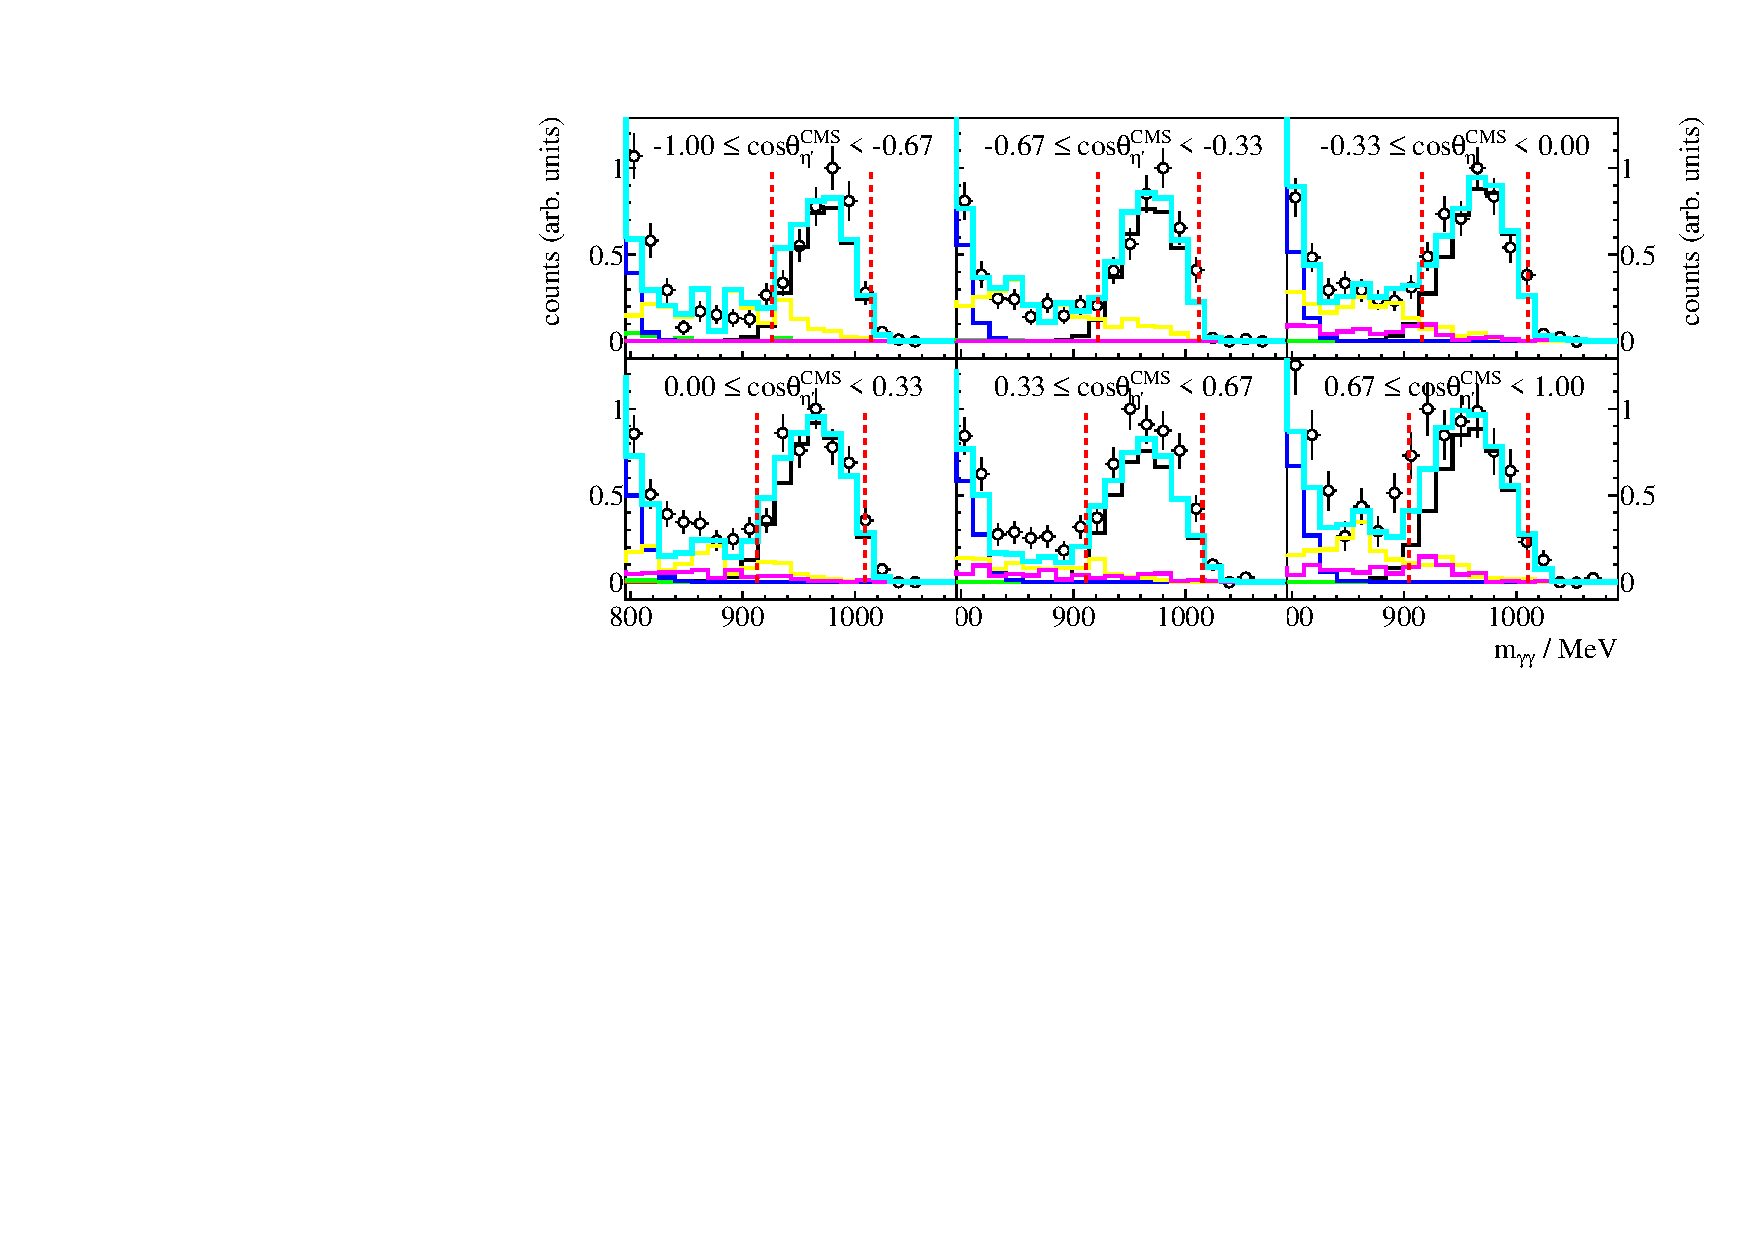
\includegraphics[width=.95\linewidth]{../../figs/hydrogen/bin_cuts/invcut_ebin1.pdf}
	data points: $m_{\gamma\gamma}$, turquoise: total MC, black: $\eta'$ MC, yellow: $2\pi^0$ MC, magenta: $\pi^0\eta$ MC, blue: $\omega$ MC
\end{frame}
\begin{frame}{Determining the beam asymmetry in $\eta'$ photoproduction}
	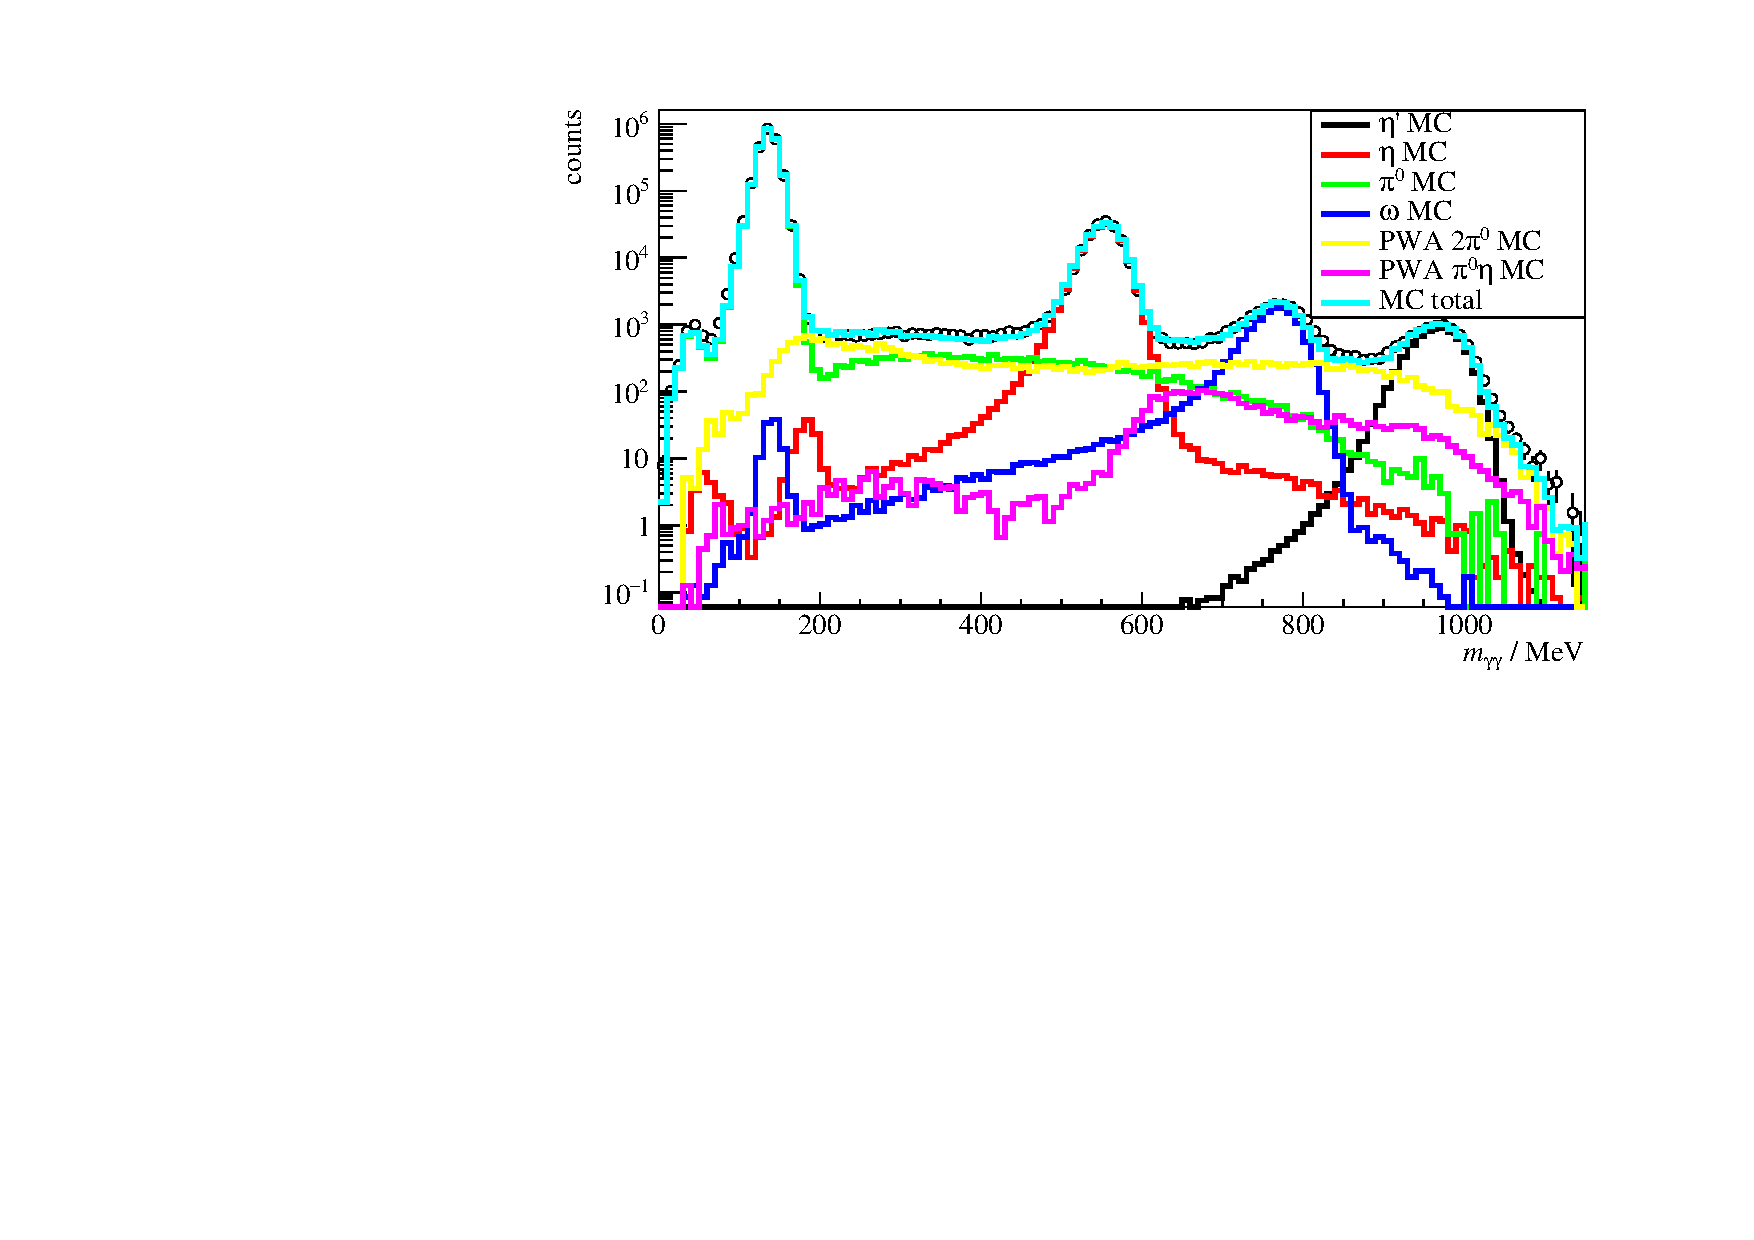
\includegraphics[width=\linewidth]{../../figs/hydrogen/invm_global.pdf}
\end{frame}
\begin{frame}{Determining the beam asymmetry in $\eta'$ photoproduction}
	Why these contributions from $4\gamma$ final states $2\pi^0$ (and $\pi^0\eta$)??
	\pause
	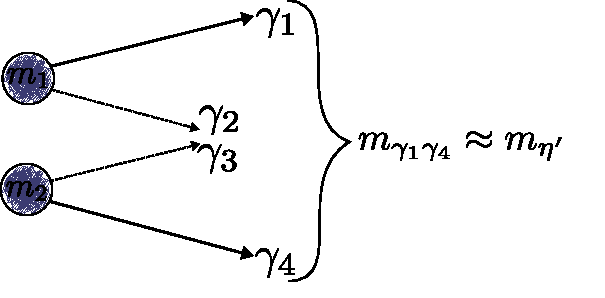
\includegraphics[width=.49\linewidth]{../../figs/inkscape/mcgammas1.pdf}
	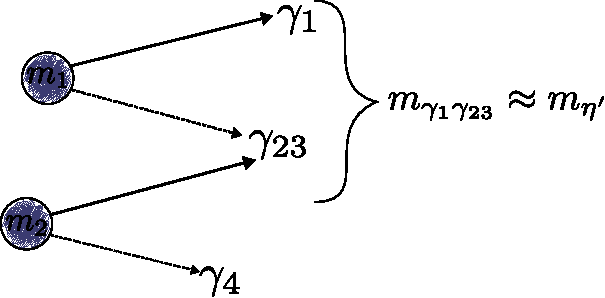
\includegraphics[width=.49\linewidth]{../../figs/inkscape/mcgammas2.pdf}
	\pause
	\emph{acceptance} for $2\pi^0$ events is almost vanishing $A(E_\gamma,\cos\theta)<2\cdot10^{-3}$, yet $$R=\frac{\sigma_{2\pi^0}\cdot\text{BR}_{2\pi^0\to\gamma\gamma}\cdot\tilde{A}_{2\pi^0}}{\sigma_{\eta'}\cdot\text{BR}_{\eta'\to\gamma\gamma}\cdot\tilde{A}_{\eta'}}=\frac{\SI{5}{\micro\barn}\cdot0.9765\cdot2\cdot10^{-3}}{\SI{1}{\micro\barn}\cdot0.023\cdot0.61}\approx0.7!$$
	explains high background contributions of up to $45\%$
	\begin{flushright}
		\cites{pdg,etap_cs,2pi0_cs}
	\end{flushright}
\end{frame}

\begin{frame}{Determining the beam asymmetry in $\eta'$ photoproduction}
	How do we get rid of background contributions?
	\begin{itemize}
		\pause
		\item simple: we don't
		\item real photons mimic a two-photon final state, no sensible additional cuts have been found
		\pause
		\item main background from $2\pi^0$ photoproduction
		\item beam asymmetry for this reaction determined by {\cites{mahlbergphd}}
		\item correct estimates for $\Sigma$ according to the amount of background
		$$\Sigma^\text{meas}=(1-\delta)\cdot\Sigma_{\eta'}+\delta\Sigma_{2\pi^0}$$
	\end{itemize}
\end{frame}
	\begin{frame}{Determining the beam asymmetry in $\eta'$ photoproduction}
		
		
		\begin{minipage}{0.49\linewidth}
			total: $\sim 8000$ $\eta'\to\gamma\gamma$ events
			\begin{itemize}
				\item perform unbinned fit as maximum likelihood fit and \textsc{Bayesian} fit
				\item \textsc{Bayesian} fit: modify likelihood
					 \begin{align*}
					 	\tilde{p}\left(\phi,\Sigma\right)&\to\tilde{p}\left(\phi,(1-\delta)\Sigma_1+\delta\Sigma_2^\text{true}\right)\\
					 	\Sigma_2^\text{true}&\sim\mathcal{N}(\Sigma_2^\text{meas},\tau)
					 \end{align*}

			\item unbinned maximum likelihood fit: shift point estimates \emph{after fit}
			\end{itemize}
		\end{minipage}
		\begin{minipage}{.49\linewidth}
			\begin{figure}
				\centering
				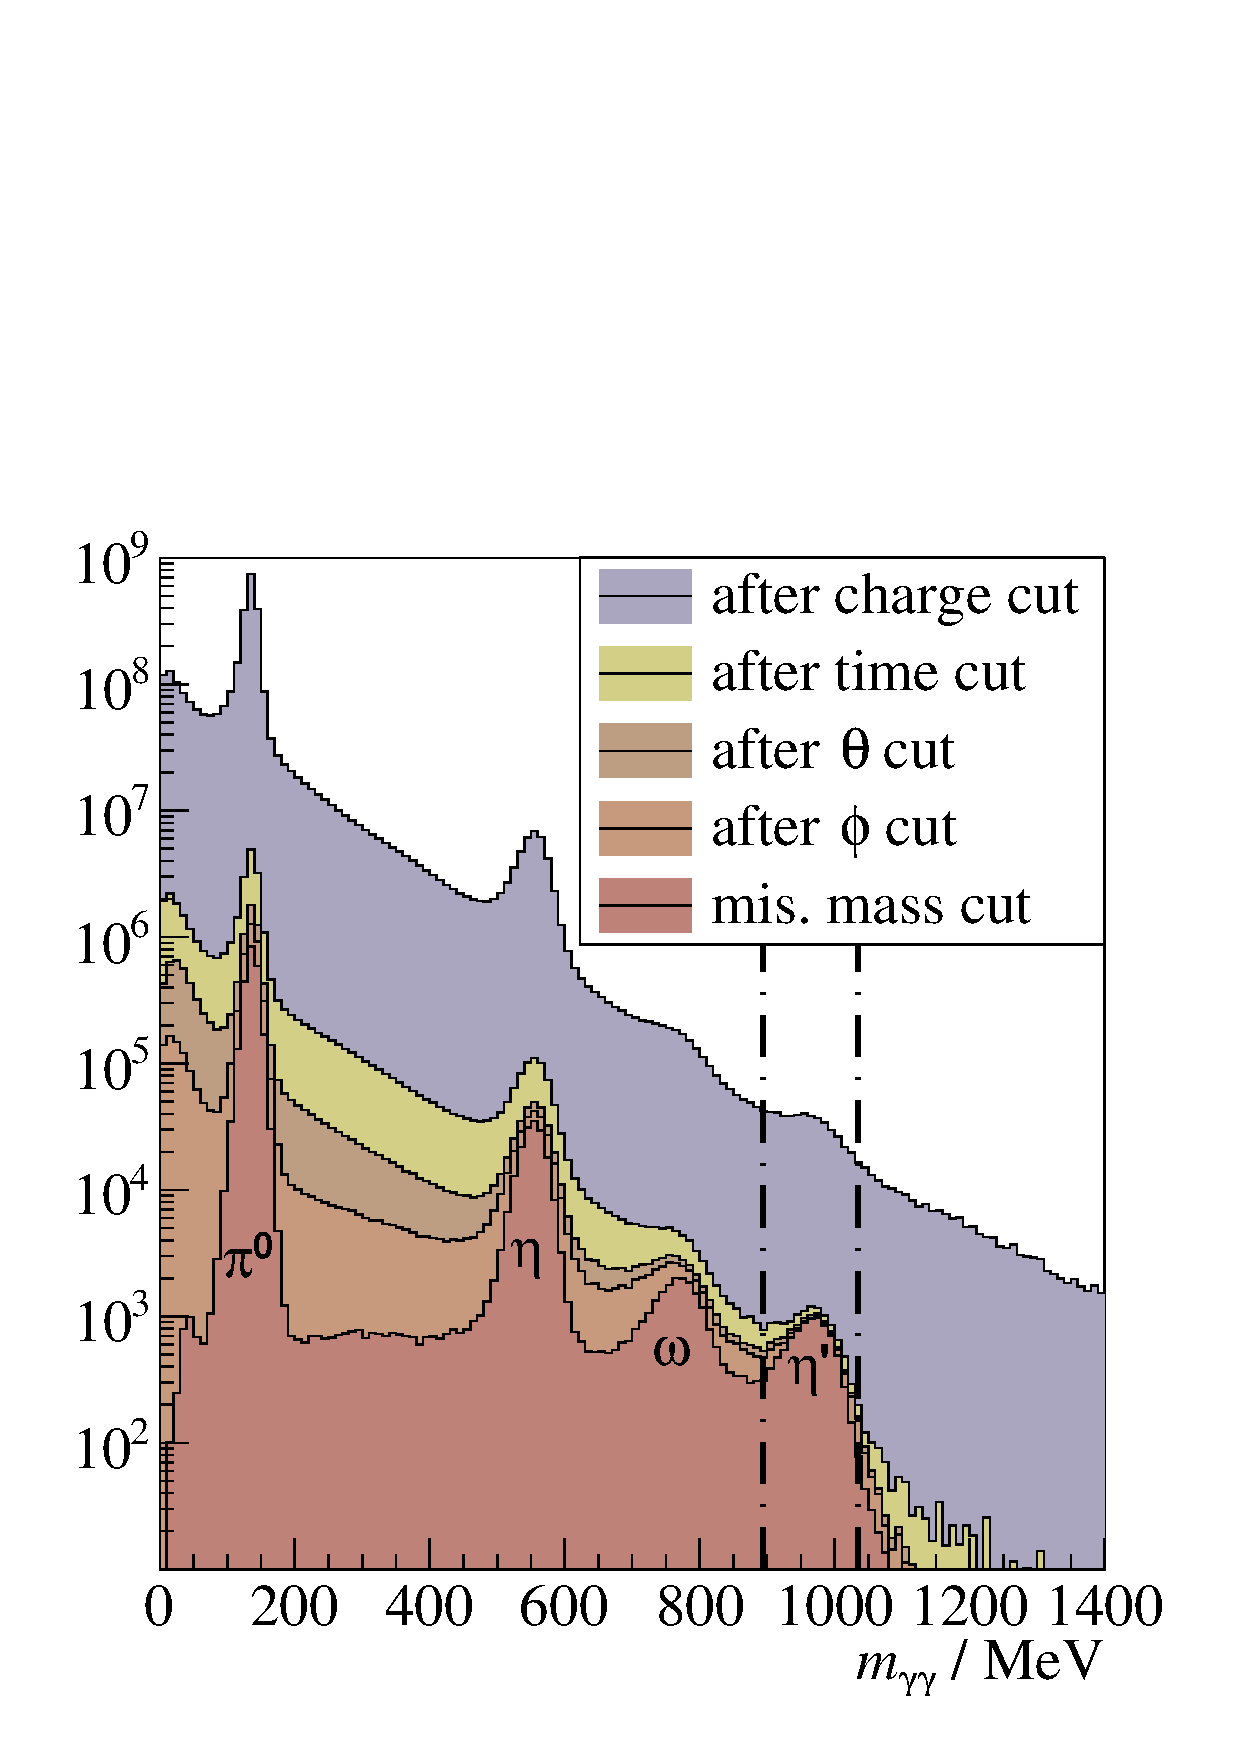
\includegraphics[width=1.05\linewidth]{../../figs/hydrogen/inc_mass_pretty_talk.pdf}
			\end{figure}
		\end{minipage}
		
	\end{frame}
	
	
	\begin{frame}{Determining the beam asymmetry in $\eta'$ photoproduction}
		\centering
		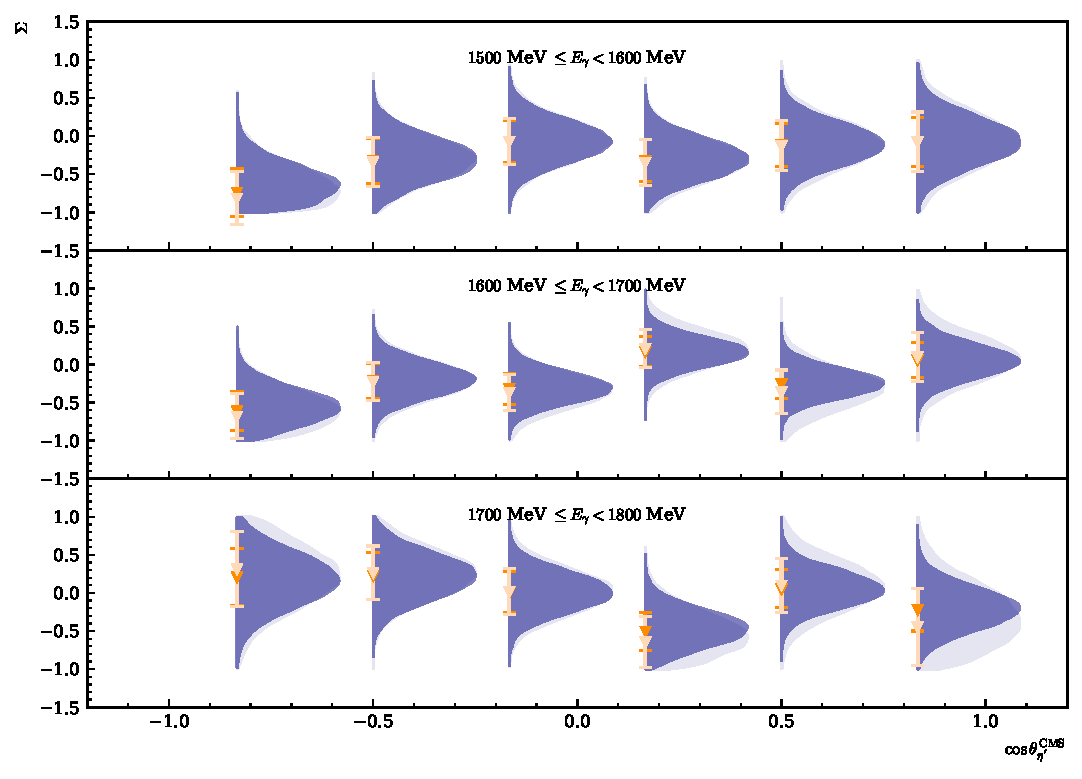
\includegraphics[width=.8\linewidth]{../../bayes/etap_event_based_fit/plots/sigma_etap_talk.pdf}
	\end{frame}
	
	
	
	
	
	\begin{frame}{Determining the beam asymmetry in $\eta'$ photoproduction}
	Systematic error: $
		\Delta\Sigma_{\eta'}^\text{sys}=\sqrt{\left(\frac{\Delta p_\gamma}{p_\gamma}\Sigma_{\eta'}\right)^2+\left(\Delta\Sigma_{\eta'}\right)^2}.$
	\begin{itemize}
		\item polarization degree \begin{equation*}
			\frac{\Delta p_\gamma}{p_\gamma}=\begin{cases}
				0.05 & E_\gamma<\SI{1600}{\mega\eV},\\ 
				0.08 & \text{ otherwise }\\
			\end{cases}
		\end{equation*}
	\item background contributions
	\begin{equation*}
		\Sigma^\text{meas}=\left(1-\delta_1-\delta_2\right)\cdot\Sigma_{\eta'}+\delta_1\Sigma_{2\pi^0}+\delta_2\Sigma^\text{r bkg},
	\end{equation*}
	thus:
	\begin{equation*}
		\Delta\Sigma_{\eta'}=\text{max}\left[\left|\frac{\Sigma^\text{meas}-\delta_1\cdot\Sigma_{2\pi^0}\pm\delta_2\cdot1}{1-\delta_1-\delta_2}-\frac{\Sigma^\text{meas}-\delta\cdot\Sigma_{2\pi^0}}{1-\delta}\right|\right]
	\end{equation*}
	\begin{flushright}
		\cites{farahphd,eberhardt_phd}
	\end{flushright}
	\end{itemize}
	\end{frame}
	\begin{frame}{Determining the beam asymmetry in $\eta'$ photoproduction}
		\begin{minipage}{.8\linewidth}
			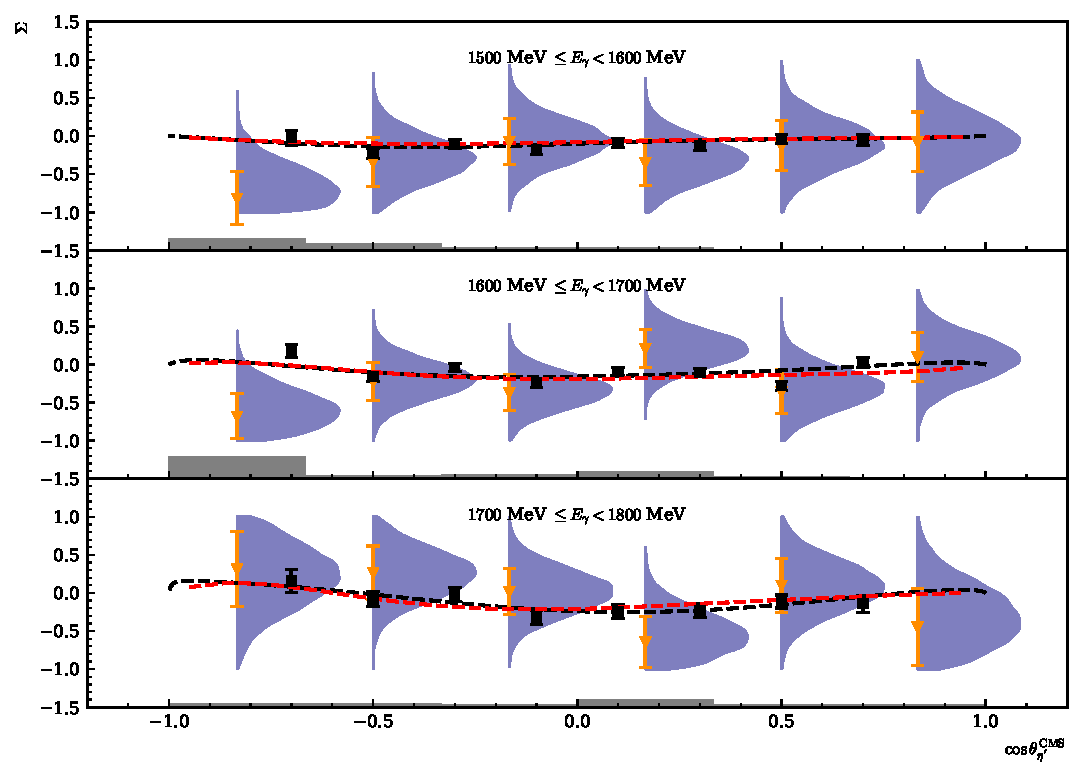
\includegraphics[width=\linewidth]{../../bayes/etap_event_based_fit/plots/sigma_etap_pwa_data_talk.pdf}
		\end{minipage}
		\begin{minipage}{.19\linewidth}
			\begin{itemize}
				{\scriptsize\item measurement at CLAS \cites{collins}: (black points),
				\item etaMAID PWA \cites{etaMAID}: (black, dashed lines),
				\item BnGa PWA \cites{etap_bnga}: (red, dashed lines)}
			\end{itemize}
		\end{minipage}
	\end{frame}

	
	
	
	\section{Conclusion}
	\begin{frame}{Conclusion}
		\begin{minipage}{.49\linewidth}
			\begin{tcolorbox}[colback=blue!5,colframe=\thecolor,title={Summary}]
				\begin{itemize}
					\item $\Sigma$ extracted for $\eta$ and $\eta'$ final state
					\item $\eta$ results obtained with \textsc{bayesian} fit agree with previous results 
					\item $\eta'$ results agree with previous measurements
				\end{itemize}
			\end{tcolorbox}
		\end{minipage}
		\begin{minipage}{.49\linewidth}
			\begin{tcolorbox}[colback=blue!5,colframe=\thecolor,title={Outlook}]
				\begin{itemize}
					
					\item use posterior \emph{distributions} for PWA calculations
					\item increase precision of existing data , i.e. investigate $\eta'\to\pi^0\pi^0\eta$
					\item measurement of observables near $\eta'$ production threshold
					
				\end{itemize}
			\end{tcolorbox}
		\end{minipage}
	\end{frame}
	
	\appendix
	\begin{frame}
		\centering
		\LARGE
		\color{\thecolor}\textsc{Backup \& References}
	\end{frame}
	\begin{frame}{Full PDF for unbinned maximum likelihood fit}
		
		\begin{align*}
			-\ln\mathcal{L}=&\sum_{i=1}^{n}-\ln(p_\text{prompt}(\phi_i,p_{\gamma,i},\Sigma,a_1\dots a_4,b_1\dots b_4))+\\
			&\sum_{j=1}^{m}-\ln\left(p_\text{sideband}(\phi_j,p_{\gamma,j},\Sigma^\text{bkg},a_1^\text{bkg}\dots a_4^\text{bkg},b_1^\text{bkg}\dots b_4^\text{bkg})\right)
		\end{align*}
		where
		\begin{align*}
			p_\text{prompt}&=f_{\text{sig}}\cdot\tilde{p}(\phi,p_\gamma,\Sigma,a_1\dots a_4, b_1\dots b_4)\\ &+ \left(1-f_\text{sig}\right)\cdot\tilde{p}(\phi,p_\gamma,\Sigma^\text{bkg},a_1^\text{bkg}\dots a_4^\text{bkg}, b_1^\text{bkg}\dots b_4^\text{bkg})\\
			p_\text{sideband}&=\tilde{p}(\phi,p_\gamma,\Sigma^\text{bkg},a_1^\text{bkg}\dots a_4^\text{bkg}, b_1^\text{bkg}\dots b_4^\text{bkg})
		\end{align*}
		and \begin{equation*}
			\tilde{p}(\phi,\Sigma)=\frac{\left(1+p_\gamma\Sigma\cos\left(2\left(\alpha^\parallel-\phi\right)\right)\right)\cdot\left(\sum_{k=0}^{4}a_k\sin(k\phi)+b_k\cos(k\phi)\right)}{1-\frac{1}{2}a_2p_\gamma\Sigma}
		\end{equation*}
		
	\end{frame}
	\begin{frame}{Additional theoretical basics}
		\begin{tcolorbox}[colback=blue!5,colframe=\thecolor,title=Unpolarized differential cross section]
			
			$$\frac{\text{d}\sigma}{\text{d}\Omega}=\frac{1}{4}\rho\sum_{\text{spins}}|\braket{f|\mathcal{F}|i}|^2\\,$$
			where
			$$\mathcal{F}=i(\vec{\sigma}\cdot\vec{\epsilon})F_1+(\vec{\sigma}\cdot\hat{q})(\vec{\sigma}\cdot(\hat{k}\times\vec{\epsilon}))F_2+i(\vec{\sigma}\cdot\hat{k})(\hat{q}\cdot\vec{\epsilon})F_3+i(\vec{\sigma}\cdot\hat{q})(\hat{q}\cdot\vec{\epsilon})F_4$$
			\begin{flushright}
				$F_i:$ complex CGLN Amplitudes
			\end{flushright}
			
			
			\begin{flushright}
				{\scriptsize[\cite{cgln}]}
			\end{flushright}
		\end{tcolorbox}
		$\frac{\text{d}\sigma}{\text{d}\Omega}\in\mathbb{R}$, not sufficient do determine $\mathcal{F}$ unambiguously\\
		$\rightarrow$ Polarization Observables can be related to $F_i$
	\end{frame}

	\begin{frame}{Diagnostics of a \textsc{bayesian} fit}
		\begin{itemize}
			\item $\hat{R}$: measure of convergence for chains
			\item Monte-Carlo-Standard-Error: measure for adequate sample size
			\item \emph{posterior predictive checks}: "goodness of fit"\\
			
		\end{itemize}
		\centering
		%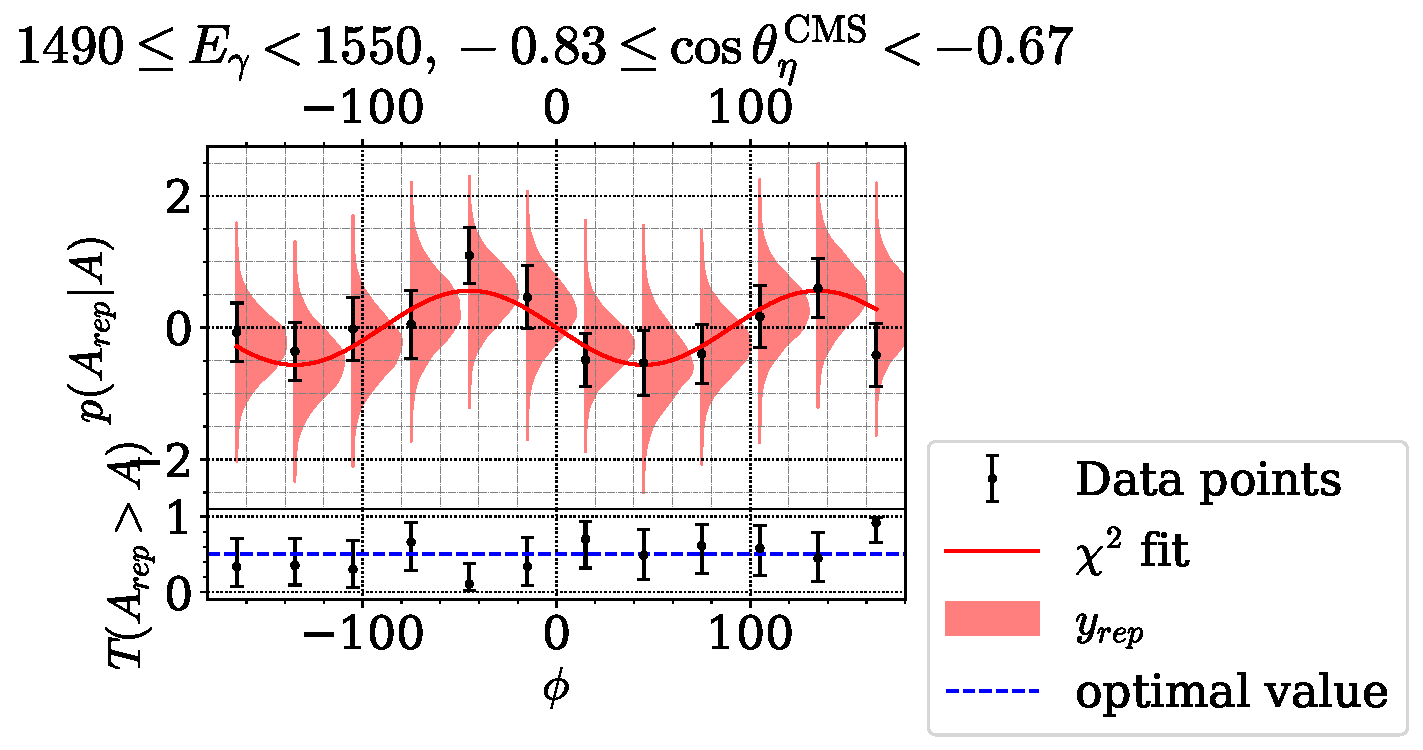
\includegraphics[width=.85\linewidth]{../bayes/realdeal/ppd_checks_alt/ebin6costbin1.pdf}
	\end{frame}
	\begin{frame}[allowframebreaks]{References}
		\printbibliography
		
	\end{frame}
	

	
\end{document}
